\documentclass[]{article}

%opening
\title{First Work in Progress}
\author{}
\usepackage{hyperref}
\usepackage{amsmath}
\usepackage[utf8]{inputenc}
\usepackage[english]{babel}
\usepackage{float}
\usepackage[caption = false]{subfig}
\usepackage[final]{graphicx}
\newtheorem{remark}{Remark}
\newtheorem{example}{Example}
\begin{document}

\maketitle

\begin{abstract}
work plan, problems and partial results
\end{abstract}

\section{Introduction}
The work has been divided in the following parts:
\begin{enumerate}
	\item Data collection
	\item Calibration
	\item Dynamic Programming (DP) Algorithm
	\item Validation 
	\item Comparisons (CPPI, constant-mix)
	\item Extensions and ideas
\end{enumerate}

\section{Details}
In this section we present what has been done so far 
\subsection{Data collection}
The three asset classes (money, bond and equity market) are represented by the following indexes:
\begin{enumerate}
	\item iShares Short Treasury Bond ETF (Money Market)
	\item BlackRock US Government Bond (Bond Market)
	\item S\&P 500 (Equity Market)
\end{enumerate}
Data were downloaded from Yahoo finance (temporary solution, Thomson Reuters will be used for the final work).
Time-series have either a daily or weekly frequency
\subsection{Calibration}
\paragraph{Gaussian model}
Asset class returns follow a Gaussian distribution ($ w_{k+1} \sim N(\mu,\Sigma)$), the calibration consists of estimating $ \mu $ and $ \Sigma $ from the data
\paragraph{Mixture model}
Two possible approaches: EM (Expectation Maximization) and MM (Method of Moments). The references for the first are (\cite{McNiel05}) while for the second are (\cite{MM93}, \cite{MM83}). I went for EM since it's already implemented in Matlab. The drowback is that it is not possible to impose an unique correlation matrix or unimodality. 
\subsection{DP Algorithm}
The general Stochastic Reachability theory is presented following \cite{Inv}.
The financial application of the algorithm is implemented following \cite{Pola2012}.
The first draft of the code can be found here: 
\url{https://github.com/skiamu/Thesis}.

As an example, we chose the following parameters:
\begin{enumerate}
	\item 2-years investment, quarterly rebalancing policy ($N=8$)
	\item target set as in \cite{PolaNonGaussian}
\end{enumerate}
The biggest challenge was the V@R constraint:
Let's define the portfolio loss as $ L = L(k,k+1):= -(x_{k+1}-x_k) $, using the relation $ x_{k+1} = x_{k}(1+u_k^{T}w_{k+1})$ we get 
\[ L = -x_{k}(u_k^T \cdot w_{k+1})\] or if we want to express the loss in return's terms we have \[ L = -(u_k^T \cdot w_{k+1})\].
In the \textbf{Gaussian case} we have that $ L \sim \mathcal{N}(\underbrace{-u^T\mu}_{\mu_p},\underbrace{u^T\Sigma u}_{\sigma_p^2})$ then \[ V@R^\Delta_{1-\alpha} = \mu_p + z_{1-\alpha} \sigma_p\] where $\Delta$ is the time horizon (in this case is the rebalancing period, 3 months).

In the \textbf{Mixture case} we need the property that linear combinations of (multivariate) Gaussian mixture are still (univariate) Gaussian mixture (see \cite{Mix05}). Therefore we have
\[\mathcal{P}(L \leq V@R_{1-\alpha}^\Delta) = 1-\alpha \quad \Rightarrow\ \mathcal{P}(-u^T w_{k+1} \leq V@R_{1-\alpha}^\Delta) = 1-\alpha     
\] since \footnote{the function $\phi_{(\mu_i,\sigma_i)}(z) $ is the normal density with mean $ \mu_i = u^T \delta_i$ and variance $ \sigma_i^2 = u^T V_i u$ where $\delta_i$ and $V_i$ are mean vector and covariance matrix of the mixture components}
\[u^T w_{k+1} \sim p_{u^T w_{k+1}}(z) = \sum_{i = 1}^{n}\lambda_i \phi_{(\mu_i,\sigma_i)}(z)\] by integration we get the CDF 
\[F_{u^T w_{k+1}}(z) = \sum_{i = 1}^{n}\lambda_i \Phi_{(\mu_i,\sigma_i)}(z)
\]
hence 
\begin{align*}
\mathcal{P}(-u^T w_{k+1} \leq V@R_{1-\alpha}^\Delta) 
&=  \mathcal{P}(u^T w_{k+1} \geq -V@R_{1-\alpha}^\Delta)\\
& = 1 - F_{u^T w_{k+1}}(-V@R_{1-\alpha}^\Delta))  \\
& = 1- \alpha
\end{align*} 
and finally \begin{center}
	\boxed{F_{u^T w_{k+1}}(-V@R_{1-\alpha}^\Delta) \leq \alpha}
\end{center}
\begin{remark}
	Let's suppose we want to impose a monthly V@R constraint, $V@R^{1m}_{99} = 7\%$. First we need to convert this V@R specification into our time horizon $\Delta = 3 m$. Using the compound rule we have \[ V@R^{3m}_{1-\alpha} = (1+V@R^{1m}_{1-\alpha})^3-1
	\] and then impose the above relation.
\end{remark}
\subsection{partial results}
The target sets were approximated in the following way:
$X_k \approx [0.5, 1.9] \quad k = 1,\ldots,7$ and $ X_8 \approx [(1+\theta)^2,1.9]$. The discretization step $\eta = 10^{-3}$, $ \theta = 7\%$, $ V@R^{1m}_{99} = 7\%$.

\begin{remark}
	The results is very sensitive to the VaR constraint, the target return $\theta$ and the distributions of the asset classes. Another method for imposing the VaR constraint can be found in (e.g. \cite{Lue13}). 
\end{remark}
\begin{remark}
	Another problem is the following: if the parameters are not carefully chosen it may happen that $J(x_0) > 1 $.
\end{remark}
Here we report the allocations maps for different time instants:
\begin{figure}[H]
	\subfloat[k = 1]{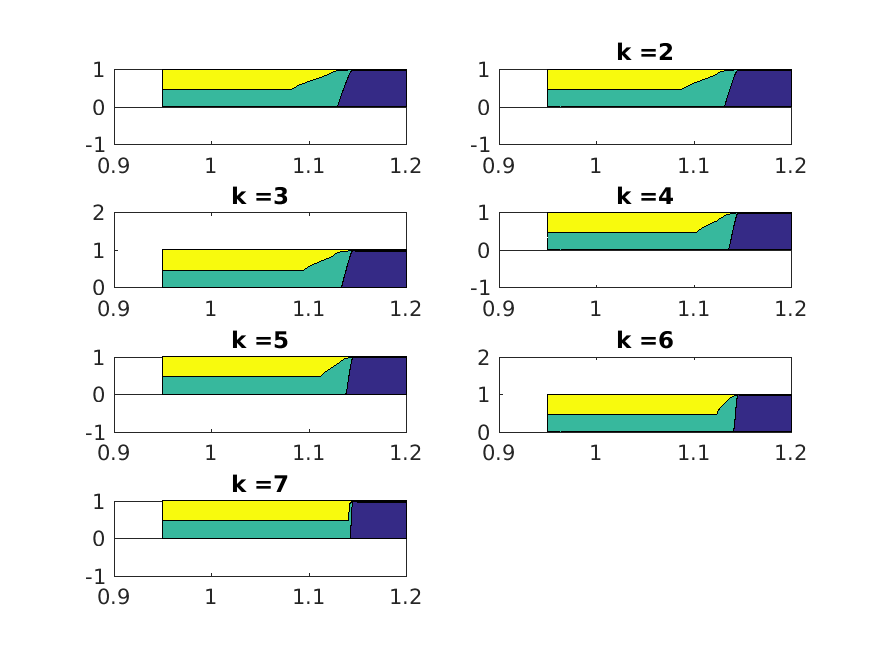
\includegraphics[width = 3in]{k1.png}} 
	\subfloat[k = 2]{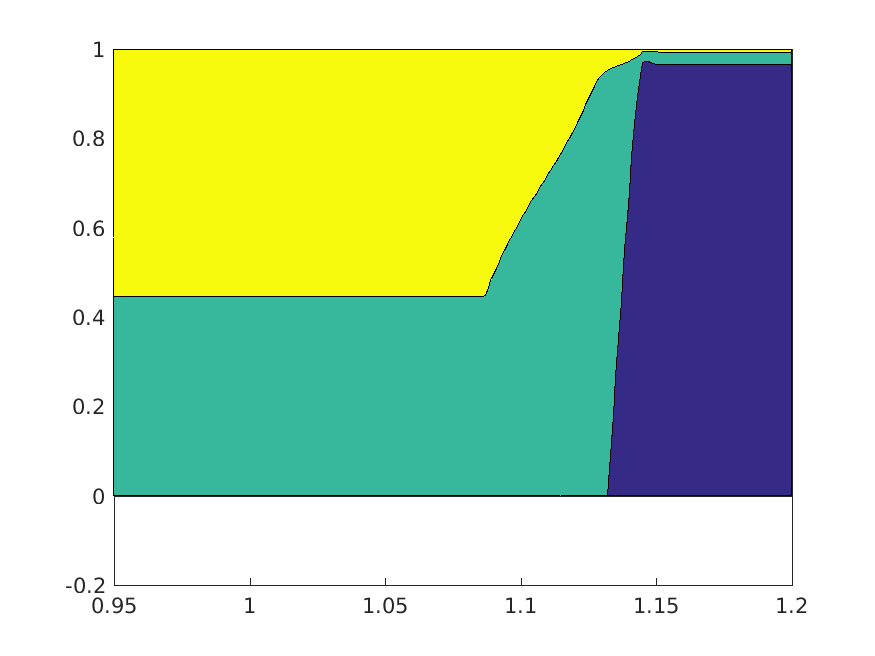
\includegraphics[width = 3in]{k2.png}}\\
	\subfloat[k = 3]{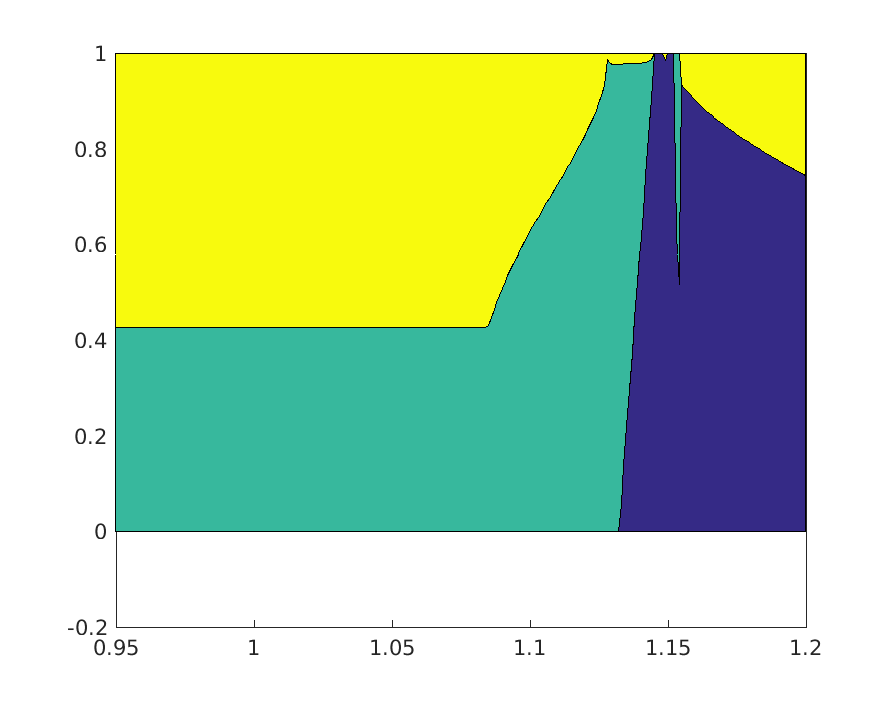
\includegraphics[width = 3in]{k3.png}}
	\subfloat[k = 4]{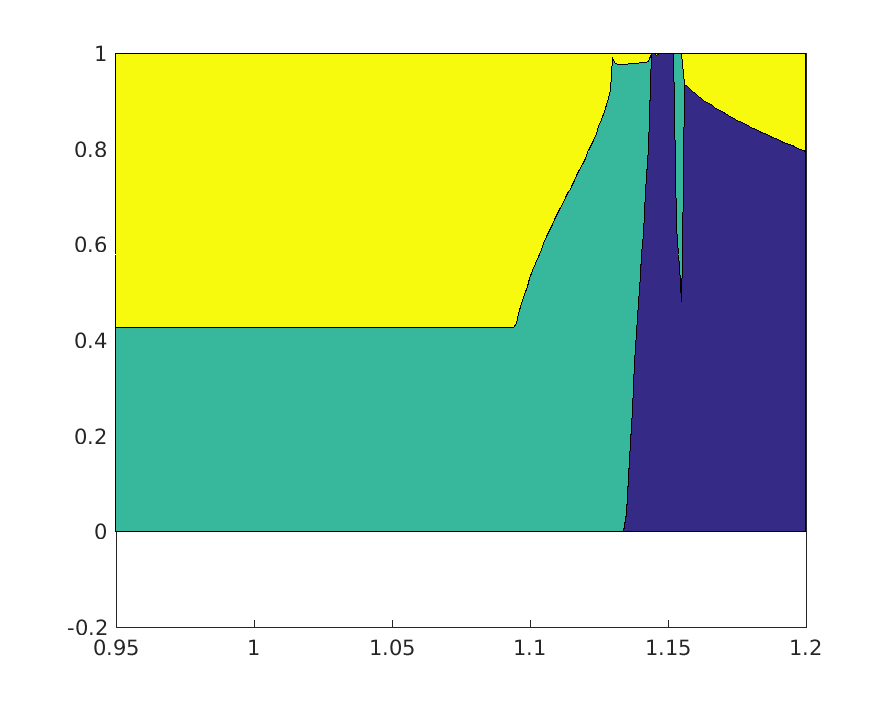
\includegraphics[width = 3in]{k4.png}} \\
	\subfloat[k = 5]{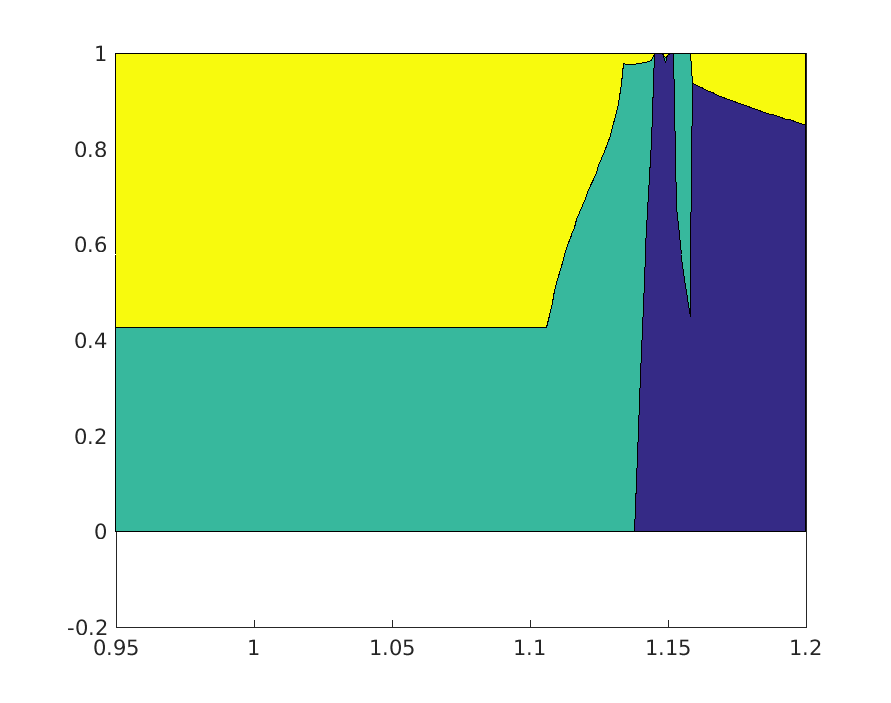
\includegraphics[width = 3in]{k5.png}}
	\subfloat[k = 6]{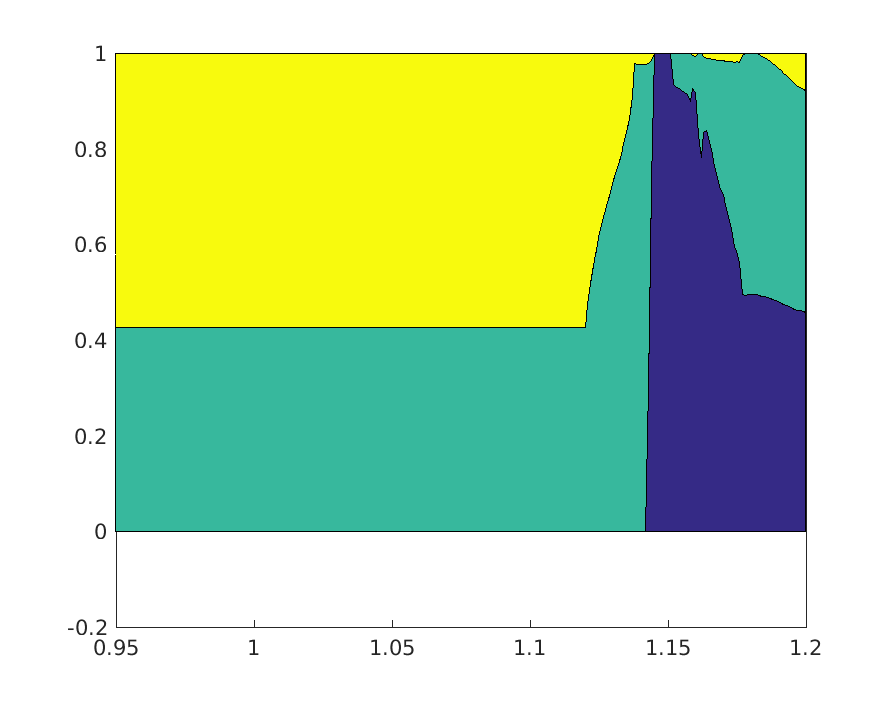
\includegraphics[width = 3in]{k6.png}} 
	
	\caption{3-months-square-root scaling rule was used of converting the VaR}
	\label{some example}
\end{figure}

\subsection{Validation}
not started yet. Simulation only at the final period or at every time step? discuss paper on mixture simulation ( I took a look at \cite{Wang01} ).
\subsection{Comparison}
not started yet
\subsection{Extensions}
\begin{itemize}
	\item Levy model for the return $ w_{k+1}$ (plus the associated calibration and simulation problem)
	\item transaction costs
	\item return estimation 
	\item Python implementation for better performance
	\item $ \dots$
\end{itemize}

\section{What next}
\begin{itemize}
	\item complete Comparison and Validation
	\item improve the code from any point of view
	\item study papers on Stochastic Hybrid System (\cite{SHS}) for possible extensions
	\item $ \dots$
\end{itemize}
\begin{thebibliography}{9}
	
	\bibitem{McNiel05}
	A. McNeil, R. Frey, P. Embrechts,
	\textit{Quantitative Risk Management},
	Princeton University Press,
	2005.
	
	\bibitem{Pola2012}
	G.Pola, G.Pola,
	\textit{A Stochastic Reachability Approach to Portfolio Construction in Finance Industry},
	2012.
	
	\bibitem{PolaNonGaussian}
	G.Pola,
	\textit{Optimal Dynamic Asset Allocation in a Non-Gaussian World}
	
	
	\bibitem{Inv}
	G.Pola, J.Lygeros, M.D. Di Benedetto,
	\textit{Invariance in Stochastic Dynamical Control Systems}
	
	\bibitem{Mix05}
	I.Buckley,D.Saunders,L.Seco,
	\textit{Portfolio optimization when asset returns have a Gaussian mixture distribution},
	European Journal of Operational Research,
	2005
	
	\bibitem{Lue13}
	David G. Luenberger,
	\textit{Investment Science},
	Oxford University Press,
	2013 second edition
	
	\bibitem{Wang01}
	Jin Wang,
	\text{Generating daily change in market variables using a multivariate mixture of normal distributions},
	2001
	
	\bibitem{MM93}
	B.G.Linsay, P.Basak,
	\text{Multivariate Normal Mixture: A Fast Method of Moments},
	Journal of the American Statistical Association,
	1993
	
	\bibitem{MM83}
	K.Fukunaga, T.Flick,
	\text{Estimation of the Parameters of a Gaussian Mixture Using the Method of Moments},
	1983
	
	\bibitem{SHS}
	A.Abate,M.Prandini,J.Lygeros,S.Sastry,
	\text{Probabilistic reachability and safety for controlled discrete time stochastic hybris systems},
	Automatica,
	2007
\end{thebibliography}

\end{document}
